\chapter{Implementation} \label{chap:implementation}

\section*{}

This chapter describes the details of implementation, in particular the architecture of the tool and the processes involved.

\section{Architecture of the solution} \label{sec:evaluation}
The architecture of this tool was subject of an intense and extensive study and deliberation in order to be implement the best solution.

The best solution would be an architecture that was flexible enough and could be easy to extended,with that the prototype to can achieve more models of assessments and consequently more practices evaluated.

The architecture of the solution can divided into two parts, its database structure and the overall application structure.

\subsection{Database structure}

This model was implemented inside of Scraim, in order to store all the information that is generated an extension of its database was done.

For that purpose several tables in the database were created. Each one one to be flexible enough to store the information of the automatic assessments.

The tables created can be viewed in the Figure \ref{fig:database}, and each purpose is:
\begin{itemize}
	\item \textbf{Model}
	
	This table contains the Models that are stored being classified only for its name, in this case the only model saved is CMMI Level 2.
	\item \textbf{Area}
	
	In this table is stored the Areas, and each Model must have one or more Areas.
	\item \textbf{Goal}
	
	Goals are part of the Area and each Area have one or more Goals.
	\item \textbf{Practice}
	
	Each Practice is a part of a Goal and can be described for its name, summary that gives a simplified description of the practice, its description which is more complete and with some examples in some cases and its weight. Each practice has different weights in the result of the assessment.
	
	\item \textbf{Practice Evaluation}
	
	Represent each Practice evaluation, each practice is evaluated with different criteria and is saved on the database for the presentation of the results.
	
	\item \textbf{Global Assessment}
	
	The Result of the assessment is represent by this table where is saved the global result, which is the aggregation of all practice evaluations for the assessment.
	
\end{itemize}

\begin{figure}[h]
	\begin{center}
		\leavevmode
		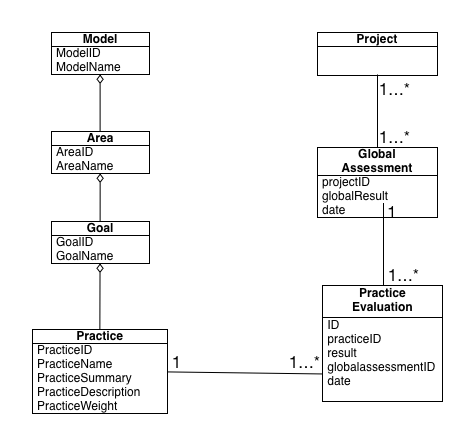
\includegraphics[width=0.8\textwidth]{ClassDiagram}
		\caption{Tables added to database}
		\label{fig:database}
	\end{center}
\end{figure}


On the left side of the Figure \ref{fig:database}, the tables represented are those who are going to be populated with the information from the CMMI for Development and in the right side is where the generated information is going to be stored.

In the Figure \ref{fig:entity-relation} is represented in a systematic way the overall interaction and process in the database, its dependencies and its flow.



\begin{figure}[h]
	\begin{center}
		\leavevmode
		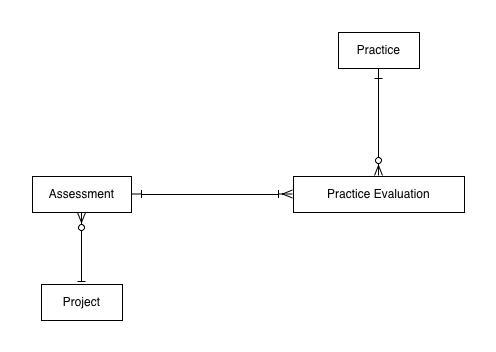
\includegraphics[width=0.6\textwidth]{Entity-Relationship-Model}
		\caption{Entity-relation model}
		\label{fig:entity-relation}
	\end{center}
\end{figure}

With this model of database was possible to achieve the goals and obtain the pretended results.

\subsection{Module Structure}



%Dar uma ideia, estrutura de criação - explicar o mvc de um modo da implementação
%Facilidade de extensão e configuração - customização (mostrar como pode ser feito)

\begin{landscape}
\begin{figure}[h]
	\begin{center}
		\leavevmode
		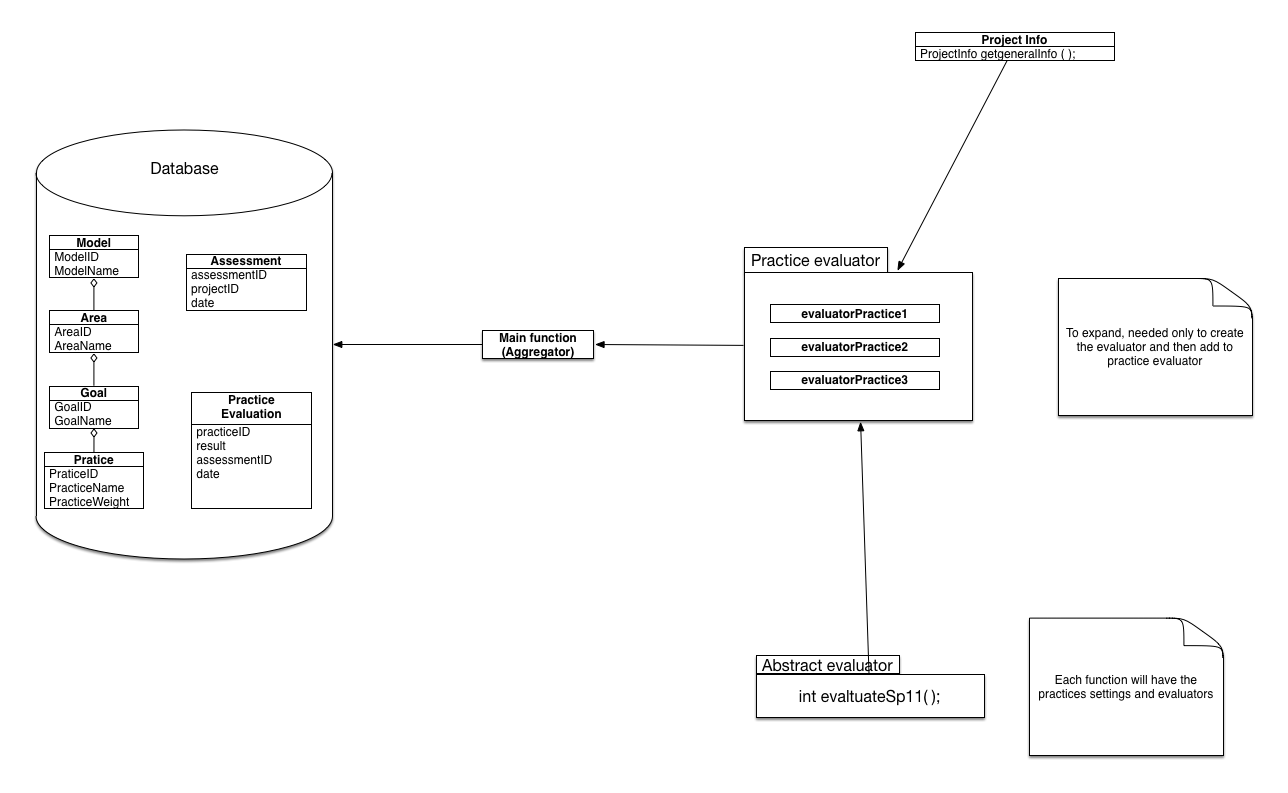
\includegraphics[width=1.2\textwidth]{esquema}
		\caption{Entity-relation model}
		\label{fig:esquema}
	\end{center}
\end{figure}
\end{landscape}

\section{CMMI coverage} \label{sec:cmmicoverage}
Scraim extension to increase cmmi coverage

